\setRL
%\pagenumbering{arabic} 
\section{
تاریخچه کوتاه
}
حاصل زحمات افراد در قرن ۱۹ و ۲۰ میلادی در راستای پی بردن به ساز و کار واحد‌های سازنده‌ی موجودات زنده، ساخت تصویری با جزئیات زیاد از سلول‌های زنده است. در سال ۱۹۸۵ ارنست اُورتن\LTRfootnote{Ernest Overton}  
سلول‌های گیاهی را در محلول‌های مختلف (قند،‌ الکل، اتر، فنول، و اَسِتُن\LTRfootnote{sugar, alcohols, ether, phenol, and acetone}) قرار داد. مشاهدات وی نشان داد که (تحت اختلاف فشار اسمزی یکسان) محلول‌هایی مانند قند که در آب به راحتی حل می‌شوند نمی‌توانند وارد سلول شوند. در صورتی که محلول‌های دیگری که حل شونده‌ی خوبی در آب نیستند، می‌توانند وارد سلول شوند. او نتیجه گرفت که جنس مرز سلول با سیتوپلاسم درون آن متفاوت است و به احتمال زیاد از ملکول‌های چربی گون تشکیل شده است
\cite{overton1985}.

در سال ۱۹۱۷ اِروین لَنگموئر \LTRfootnote{Irving Langmuir}
 مقاله‌ای چاپ کرد که در آن روشی برای اندازه‌گیری فشار جانبی\LTRfootnote{lateral}
 غشا در سطح مقطع مشترک هوا و آب پیشنهاد داد
 \cite{Langmuir1917}.
 او با استفاده از روش خود نشان داد که غشا در این سطح مقطع مشترک یک تک لایه‌ی ملکول چرب تشکیل می‌دهد و مساحت هر ملکول را 
 $S_{lipid} = 0.7 nm^2$
 گزارش کرد. او همچنین در گزارش خود پیشنهاد داد که غشا از ملکول‌های دوزیست\LTRfootnote{Amphiphiles}
 تشکیل شده. ملکول‌های دوزیست به ملکول‌هایی گفته می‌شود که یک گروه سَر دو قطبی آب‌دوست و یک یا چند دُم هیدروکربنی آب‌گریز داشته باشد. 
 
 با به کارگیری روش اندازه‌گیری لنگموئر، در سال ۱۹۲۵، گُرتِر\LTRfootnote{E. Gorter}
 و گرِندِل\LTRfootnote{F. Grendel}
 نشان دادند که  غشای گلبول‌های قرمز از یک دو-لایه لیپید تشکیل شده
 \cite{Gorter1925}.
 آن‌ها غشای گلبول را در اَسِتُن حل کرده و با روش لنگموئر سطح آن را اندازه‌گیری کردند. سپس این عدد را با مساحت گلبول قرمز خشک شده مقایسه کردند. در آزمایش آن‌ها دو خطا وجود داشت؛ اولین خطا در اینجا بود که اَسِتُن نمی‌تواند تمام ملکول‌های چربی را از گلبول جدا کند، و دوم در اندازه‌گیری مساحت گلبول قرمز بود
 \cite{BiomembranesBook1989,BioMemBook2007}.
 ولی خوشبختانه این دو خطای اندازه‌گیری همدیگر را تکمیل کردند و آن‌ها نسبت این دو عدد را با تقریب خوبی نزدیک به ۲ اندازه‌گیری کردند که با اطلاعات فعلی ما از ساختار  دو-لایه غشای گلبول قرمز سازگار است
 \cite{Edidin2003}.
 
  
 
 
 در سال ۱۹۳۲ (حدود نود سال پیش) کِنِت کول\LTRfootnote{Kenneth Cole}
 تخم جوجه‌تیغی دریایی\LTRfootnote{sea urchin (arbacia) egg} 
را بر سطحی قرار داد و  با کمک یک فیبرِ از جنس طلا به تخم  فشار وارد کرد. با اندازه‌گیری  کشش سطحی و مقایسه‌ی آن با حد تحمل فشار تخم، استدلال کرد که لایه‌ی نازکی که در اطراف سلول وجود دارد تنها از ملکول‌های چربی درست نشده است
 \cite{Cole1932}. 

در دهه‌ی ۱۹۳۰ داوسن\LTRfootnote{H. Davson} 
و دنیِلی\LTRfootnote{J. F. Danielli} 
مدل جدیدی برای غشا پیشنهاد دادند. آن‌ها با آزمایش بر روی غشا‌های مصنوعی و سلولی، دلیل اختلاف در تراوایی دو روی غشا در عبور مواد یونی و دوقطبی را وجود لایه‌ای از پروتئین بر روی غشا توصیف کردند
\cite{Danielli1935}. 
این مدل غشا اولین مدلی بود که به طور عمومی پذیرفته  و تا سال‌ها  در تحقیقات استفاده شد. حتی پس از  پدید آمدن ابزار‌های تصویر‌برداری دقیق، این مدل تنها با کمی تغییر جزئی مواجه شد.

در دهه‌ی ۱۹۵۰ با فرا رسیدن تکنولوژی میکروسکوپ الکترونی، رابرتسون\LTRfootnote{J. D. Robertson}
 اولین تصاویر از غشای سلول را رونمایی کرد. وی با استفاده از روش‌های رنگ آمیزی، وجود لیپید‌ها\LTRfootnote{lipid}
 در غشا را تایید و ضخامت غشای سلولی را بین ۵ تا ۱۰ نانومتر اندازه‌گیری کرد
\cite{ROBERTSON1959aa}.
او همچنین نشان داد که غشای پلاسمایی و تمامی اعضای غشاگون مثل غشای هسته‌ی سلول و غشای دو-لایه میتوکندریا\LTRfootnote{mitochondria}
ساختار مشترکی دارند که مدل داوسن-دنیلی و مشاهدات گُرتِر و گرِندِل را تایید می‌کرد.
همچنین درنتیجه‌ی اندازه‌گیری با میکروسکوپ و پراش اشعه‌ی X ضخامت غشا 
 $5-8nm$
و ضخامت لایه‌ی مرکزی آبگریز آن
 $3-4nm$
گزارش شد
\cite{NelsonBook2004}.
با پیشرفت سریع روش‌های اندازه‌گیری و تصویربرداری بر پایه‌ی تشدید مغناطیسی (مانند تشدید مغناطیسی‌ هسته‌ای یا NMR\LTRfootnote{nuclear magnetic resonance}
و تشدید اسپین الکترون\LTRfootnote{electron spin resonance}) آزمایش‌های زیادی طراحی شد که نشان داد غشا  خواصی شبیه به مایع دارد
\cite{Edidin2003}
و لیپید‌ها می‌توانند بر سطح غشا با ضریب پخش
$D_{lipid}\sim 10^{-8}cm^2/s\approx 10^6S_{lipid}/s$
 حرکت کنند
\cite{NelsonBook2004,Chapman1975}.
همچنین عدم تقارن بین دولایه‌ی غشا تایید شد و برای اولین بار با علامت گذاری پروتئین‌های بر روی دو سطح غشا، حضور پروتئین‌ها در درون غشا نشان داده شد
\cite{Bretscher1973}.



افراد زیادی در تکمیل شدن تصویری که امروزه از غشای سلول وجود دارد نقش داشتند، ولی تصویر مدرن ما از غشاهای سلول‌ها بیشتر بر پایه‌ی مدل غشای مایع موزایکی‌\LTRfootnote{the mosaic fluid model of membranes}
 است که در سال ۱۹۷۲ توسط سینگر\LTRfootnote{Singer}
  و نیکلسون\LTRfootnote{Nicholson}
 ارائه شد
\cite{Singer1972}
(شکل 
\ref{fig:fluidmembranemodel}). بنا بر این مدل، غشا را می‌توان یک مایع همگن دو بعدی وُشکسان از چربی‌ها و کُلِسترول فرض کرد که ماکرو-ملکول‌های پروتئینی به کمک برهمکنش‌های آب‌گریز  بر روی سطح یا درون آن قرار گرفته و کم و بیش آزادانه حرکت می‌کنند (مانند دریای قطب شمال و تکه‌های یخ  شناور در آن).  در نتیجه هیچ نظم بلند بردی در غشا دیده نمی‌شود. 

\begin{figure}[h]
\begin{center}
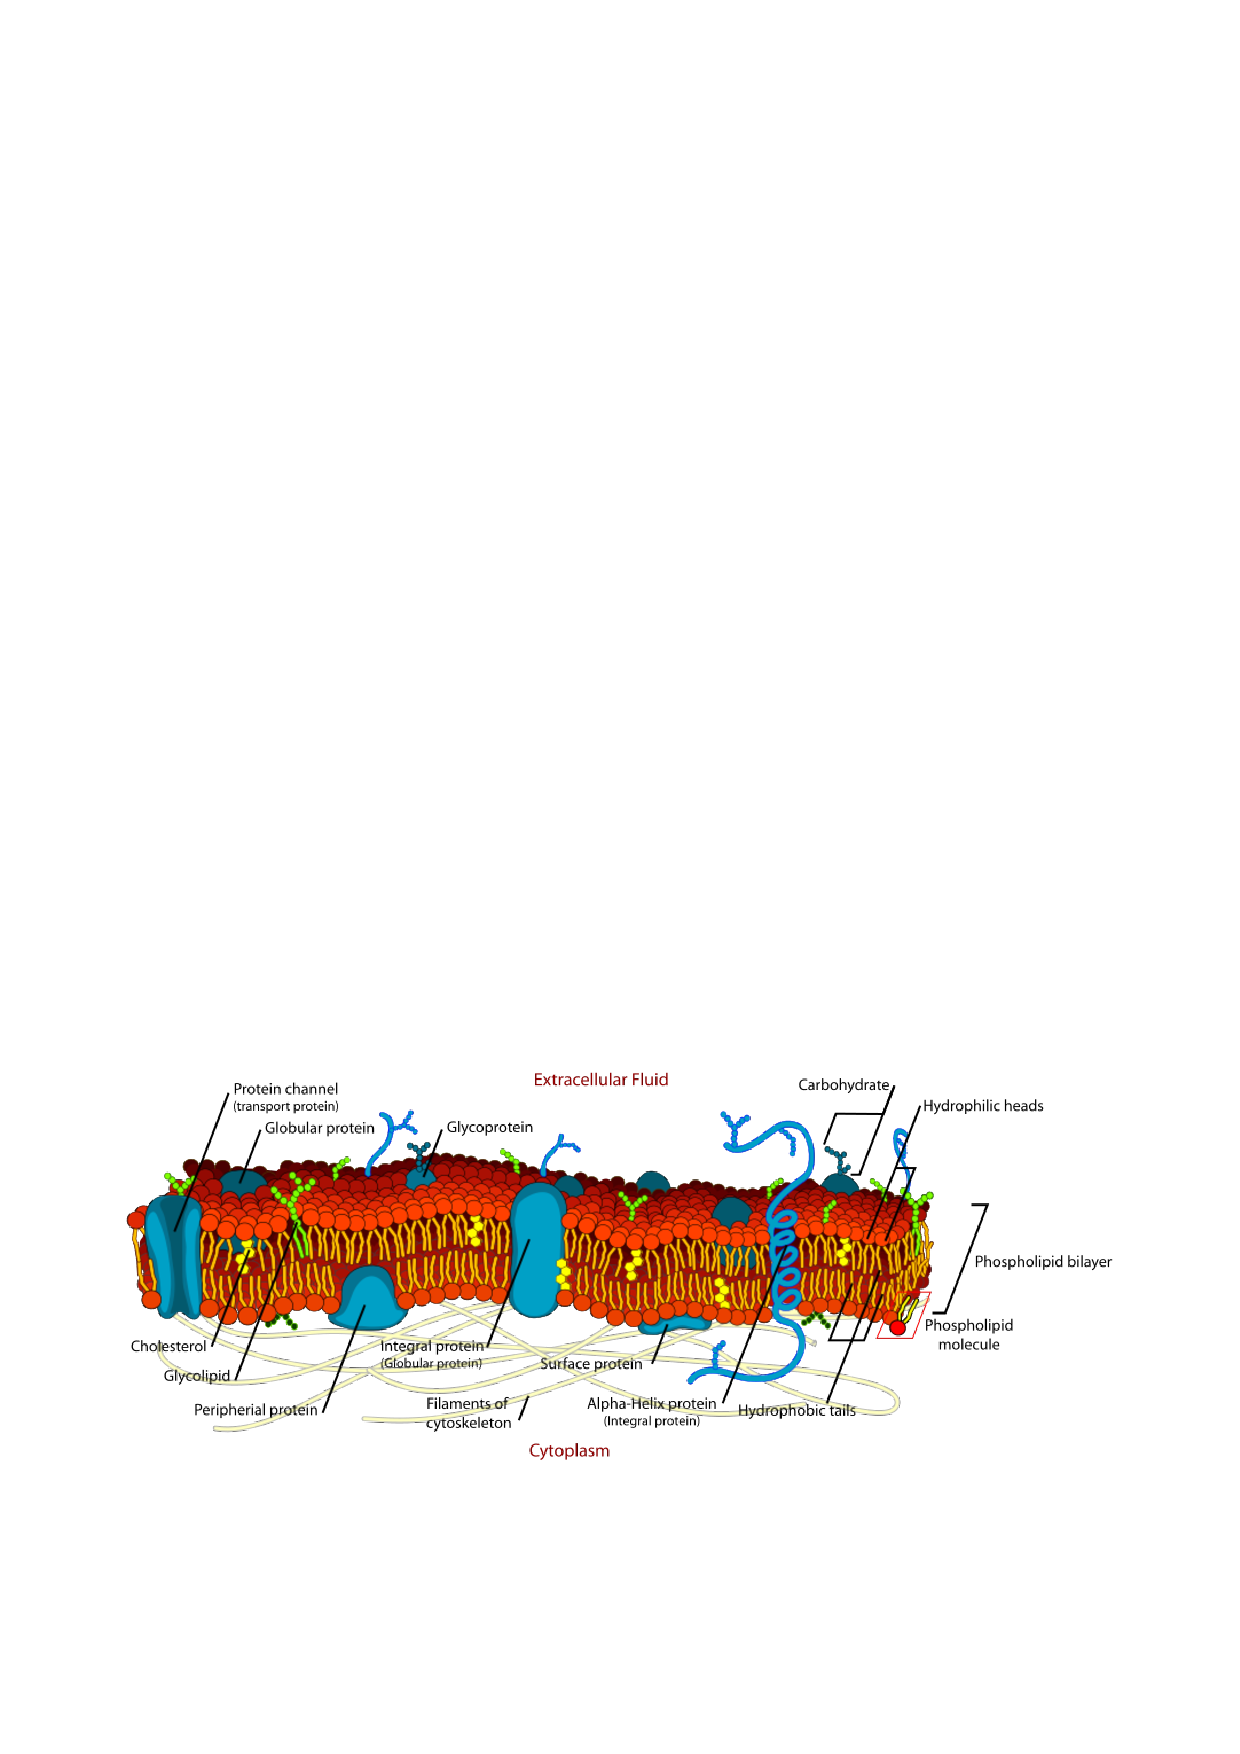
\includegraphics[width=6in]{\MemBio /Pics/Cell_membrane_detailed_diagram}
\caption{
شکل از سایت ویکیپیدیا گرفته شده است
\cite{wikiCellMembrane}. این یک نقاشی از غشا بر اساس مدل غشای مایع موزایکی است. بیشتر غشا از ملکول‌های چربی تشکیل شده ولی پروتئین‌های خیلی زیادی نیز در غشا قرار دارد.  غشا از طریق این پروتئین‌ها به اسکلت سلولی و اجزای دیگر متصل است. دایره‌های قرمز سر آب‌دوست و رشته‌های زرد دُم‌های آب‌گریز لیپید‌ها را نشان می‌دهد.
}
\label{fig:fluidmembranemodel}
\end{center}
\end{figure}


در نتیجه‌ی توسعه‌ی تحقیقات، می‌دانیم غشا‌های زیستی بیشتر ساختار موزائیکی دارند تا مایع. یعنی در سلول‌های مختلف غشا خیلی همگن نیست و در یک سلول قسمت‌هایی از غشا ممکن است  ترکیب پروتئینی متفاوتی از بخش‌های دیگر همان سلول داشته باشد. همچنین ضخامت برخی از بخش‌های غشا ممکن است از چند ۱۰ نانومتر تا ۱۰۰ نانومتر (که با سفینگولیپید\LTRfootnote{sphingolipids}
و کُلِسترول غنی است) تغییر کند
\cite{Engelman:2005aa}. یکی از دلایل غیر همگن بودن غشا نامتقارن شدن آن به علت حضور قسمت میانی آب‌گریز غشا در کنار پروتئین‌ها یا پلی‌پپتیدها\LTRfootnote{polypeptide}
است.  مرکز غشا از نواری از دم‌های آب‌گریز تشکیل شده. پروتئینی هم که درون غشا قرار گرفته قسمت آبگریز خود را درون غشا جا داده و قسمت آب‌دوستش را بیرون. کافی‌است که قسمت آب‌گریز پروتئین  کمی از ضخامت نوار آب‌گریز لیپید‌های  بیشتر یا کمتر باشد که ضخامت غشا را تغییر دهد
\cite{Mouritsen1984}. 
در این حالت یا پروتئین باید تغییر شکل دهد که خود را با ضخامت غشا تنظیم کند، یا هر دو (شکل 
\ref{fig:BilayerPlusProtein}) که در هر حالت باعث بروز برهمکنش‌‌های پروتئین-لیپید و لیپید-لیپید می‌شود
\cite{Huang1986,Aranda-Espinoza1996,Safran2000,Haselwandter2013,Haselwandter-Christoph2013}.
مدل موزائیکی مدل خوبی است که مشکلات حرکتی لیپید‌ها و پروتئین‌های چسبیده به غشا را توضیح می‌دهد
\cite{Simons2000,Simons1997}.


\begin{figure}[h]
\begin{center}
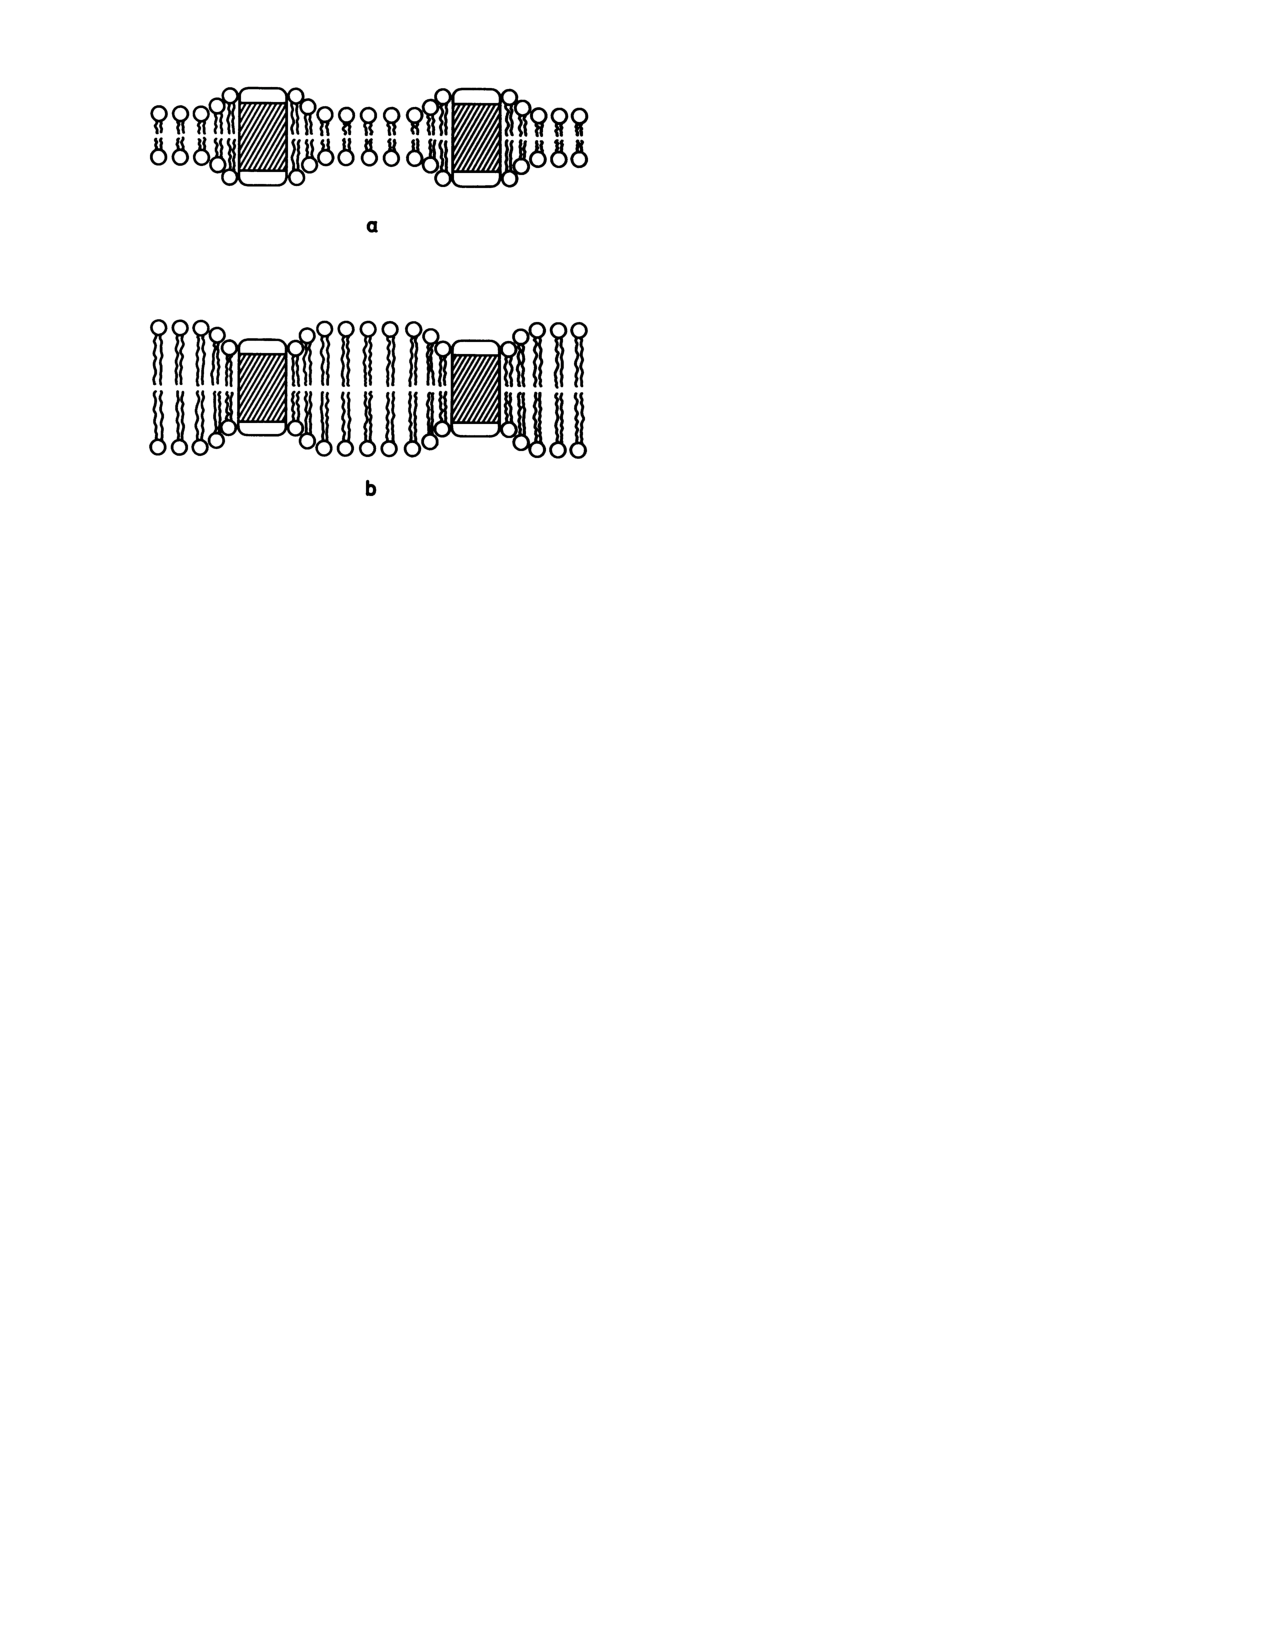
\includegraphics[width=4in]{\MemBio /Pics/BilayerPlusProtein}
\caption{
نقاشی از برش یک غشای لیپیدی که حاوی نوعی ناخالصی (مانند پروتئین یا پلی‌پپتید) است. ملکول‌های لیپید با دایره‌های سفید (سر آب‌دوست) و دم‌های آب‌گریز، و  ناخالصی‌ها به شکل مستطیل‌های دارای سر‌های آب‌دوست و ناحیه‌ی میانی هاشور خورده‌ی آب‌گریز نمایش داده شده‌است. اگر ناحیه‌ی آب‌گریز ناخالصی نسبت به غشا ضخیم‌تر (الف) یا نازک‌تر (ب) باشد، ضخامت غشا تحت تاثیر قرار می‌گیرد
\cite{Mouritsen1984}
.
}
\label{fig:BilayerPlusProtein}
\end{center}
\end{figure}





با وجود اینکه غشای لیپیدی به طور خود سامانده تشکیل می‌شود ولی علاوه بر ملکول‌های چربی پروتئین‌های زیادی نیز به غشا ساختار می‌بخشد
\cite{wikiCellMembrane}. غشاهایی هم می‌توان یافت که درصد پروتئین و کربوهیدارت در ساختار  آن به ترتیب بین ۱۸ تا ۷۵ درصد و  ۳ تا ۱۰ درصد باشد
\cite{MembraneProteins1972}. 
غشا از طریق این پروتئین‌ها به اجزای پیچیده‌تر داخل سلول (مانند اسکلت سلولی) متصل است. خاصیت تراوایی فوسفولیپید دو لایه و کانال‌های پروتئینی درون غشا، ارتباط سلول با محیط اطراف را کنترل و مدیریت می‌کند.  

